\documentclass{beamer}

\mode<presentation> {

% La clase Beamer tiene varios temas predeterminados disponibles para las diapositivas.

%\usetheme{default}
%\usetheme{AnnArbor}
%\usetheme{Antibes}
%\usetheme{Bergen}
%\usetheme{Berkeley}
%\usetheme{Berlin}
%\usetheme{Boadilla}
%\usetheme{CambridgeUS}
%\usetheme{Copenhagen}
%\usetheme{Darmstadt}
\usetheme{Dresden}
%\usetheme{Frankfurt}
%\usetheme{Goettingen}
%\usetheme{Hannover}
%\usetheme{Ilmenau}
%\usetheme{JuanLesPins}
%\usetheme{Luebeck}
%\usetheme{Madrid}
%\usetheme{Malmoe}
%\usetheme{Marburg}
%\usetheme{Montpellier}
%\usetheme{PaloAlto}
%\usetheme{Pittsburgh}
%\usetheme{Rochester}
%\usetheme{Singapore}
%\usetheme{Szeged}
%\usetheme{Warsaw}

% Junto a los temas, Beamer también cuenta con variaciones de colores y fuentes.

%\usecolortheme{albatross}
%\usecolortheme{beaver}
%\usecolortheme{beetle}
%\usecolortheme{crane}
%\usecolortheme{dolphin}
%\usecolortheme{dove}
%\usecolortheme{fly}
%\usecolortheme{lily}
%\usecolortheme{orchid}
%\usecolortheme{rose}
%\usecolortheme{seagull}
%\usecolortheme{seahorse}
%\usecolortheme{whale}
%\usecolortheme{wolverine}
}

% Núcleo
\usepackage[utf8]{inputenc}
\usepackage[spanish]{babel}

% Gráficos
\usepackage{graphicx}
\usepackage{booktabs}


% El título corto aparece en la parte inferior de cada diapositiva.
% El título completo solo en la página de título
\title[Plataforma de iniciación en la ciberseguridad]
{Diseño e implementación de una plataforma web de iniciación en la ciberseguridad}

% Nombre del autor
\author{Antonio Javier Galán Herrera}

% Institución a la que perteneces.
% Aparecerá en la parte inferior de cada diapositiva.
% Puede ser abreviado para ahorrar espacio
\institute[ETSII]
{Escuela Técnica Superior de Ingeniería Informática}

\date{\today}


\begin{document}

\begin{frame}
    \titlepage
\end{frame}

\begin{frame}{Índice}
    \tableofcontents
\end{frame}


\section{Introducción}

    \begin{frame}
        \Huge{\centerline{Introducción}}
    \end{frame}

    \begin{frame}{Motivación}
        \begin{itemize}
            \item Estrategia Andaluza de Ciberseguridad 2022 - 2025
            \\~\\
            \item Proyecto para estudiantes, desarrollado por un estudiante
            \\~\\
            \item Algo distinto a los CTFs, sin \textit{banderas}
        \end{itemize}
    \end{frame}

    \begin{frame}{Metodología}
        \begin{columns}[c]
            \column{.45\textwidth}
                \begin{itemize}
                    \item Desarrollo incremental
                    \\~\\
                    \item \textit{Getting Things Done}
                    \\~\\
                    \item Gantt y Kanban
                \end{itemize}
            
            \column{.5\textwidth}
                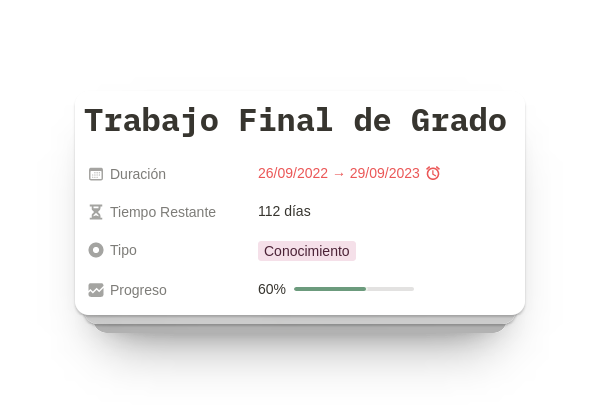
\includegraphics[scale=0.25]{images/capturas/notion.png}
        \end{columns}
    \end{frame}

    \begin{frame}{Proceso creativo}
        \begin{columns}[c]
            \column{.45\textwidth}
                \begin{itemize}
                    \item Plataforma de CTFs
                    \\~\\
                    \item Portal de descargas
                    \\~\\
                    \item \textbf{Laboratorios}
                \end{itemize}
            
            \column{.5\textwidth}
                
\includegraphics[scale=0.25]{images/interrogacion.png}
        \end{columns}
    \end{frame}

    \begin{frame}{Análisis de tecnologías}
        \begin{itemize}
            \item \textbf{Sitio web}: Astro / WordPress / Drupal
            \\~\\
            \item \textbf{Base de datos}: SQLite / MySQL
            \\~\\
            \item \textbf{Almacenamiento}: Local / Remoto (AWS, Linode, GCP) 
        \end{itemize}
    \end{frame}


\section{Diseño y desarrollo}

    \begin{frame}
        \Huge{\centerline{Diseño y desarrollo}}
    \end{frame}

    \begin{frame}{Arquitectura}
        \centering

        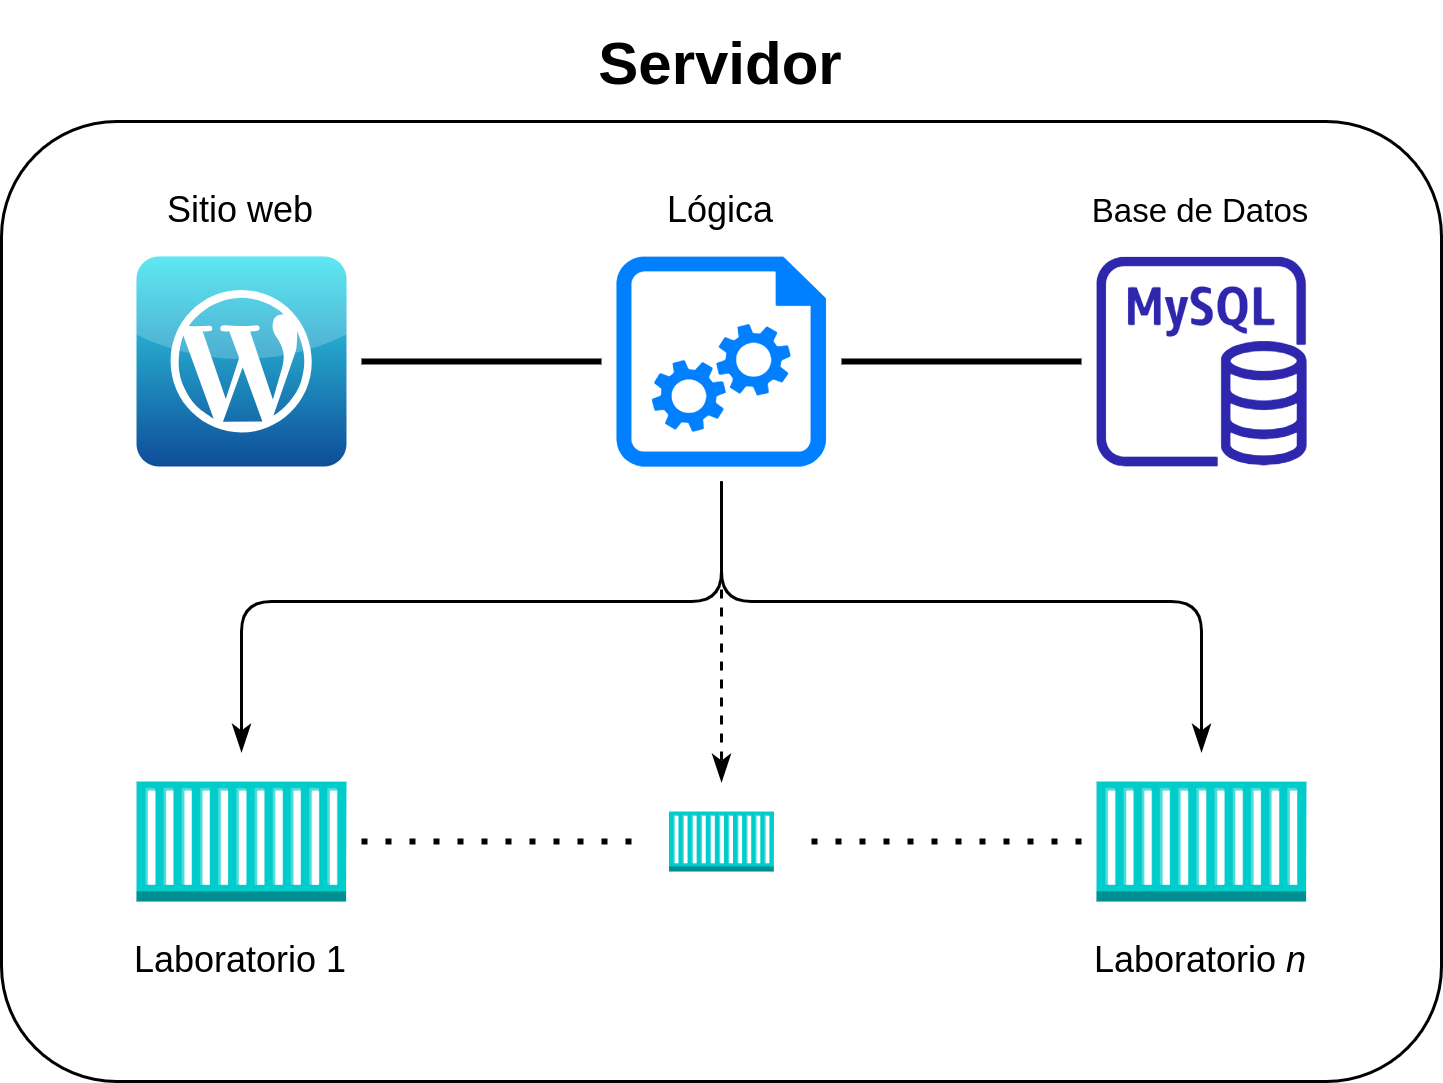
\includegraphics[scale=0.15]{images/diagramas/arquitectura.png}
    \end{frame}

    \begin{frame}{Modelado de procesos}
        \centering

        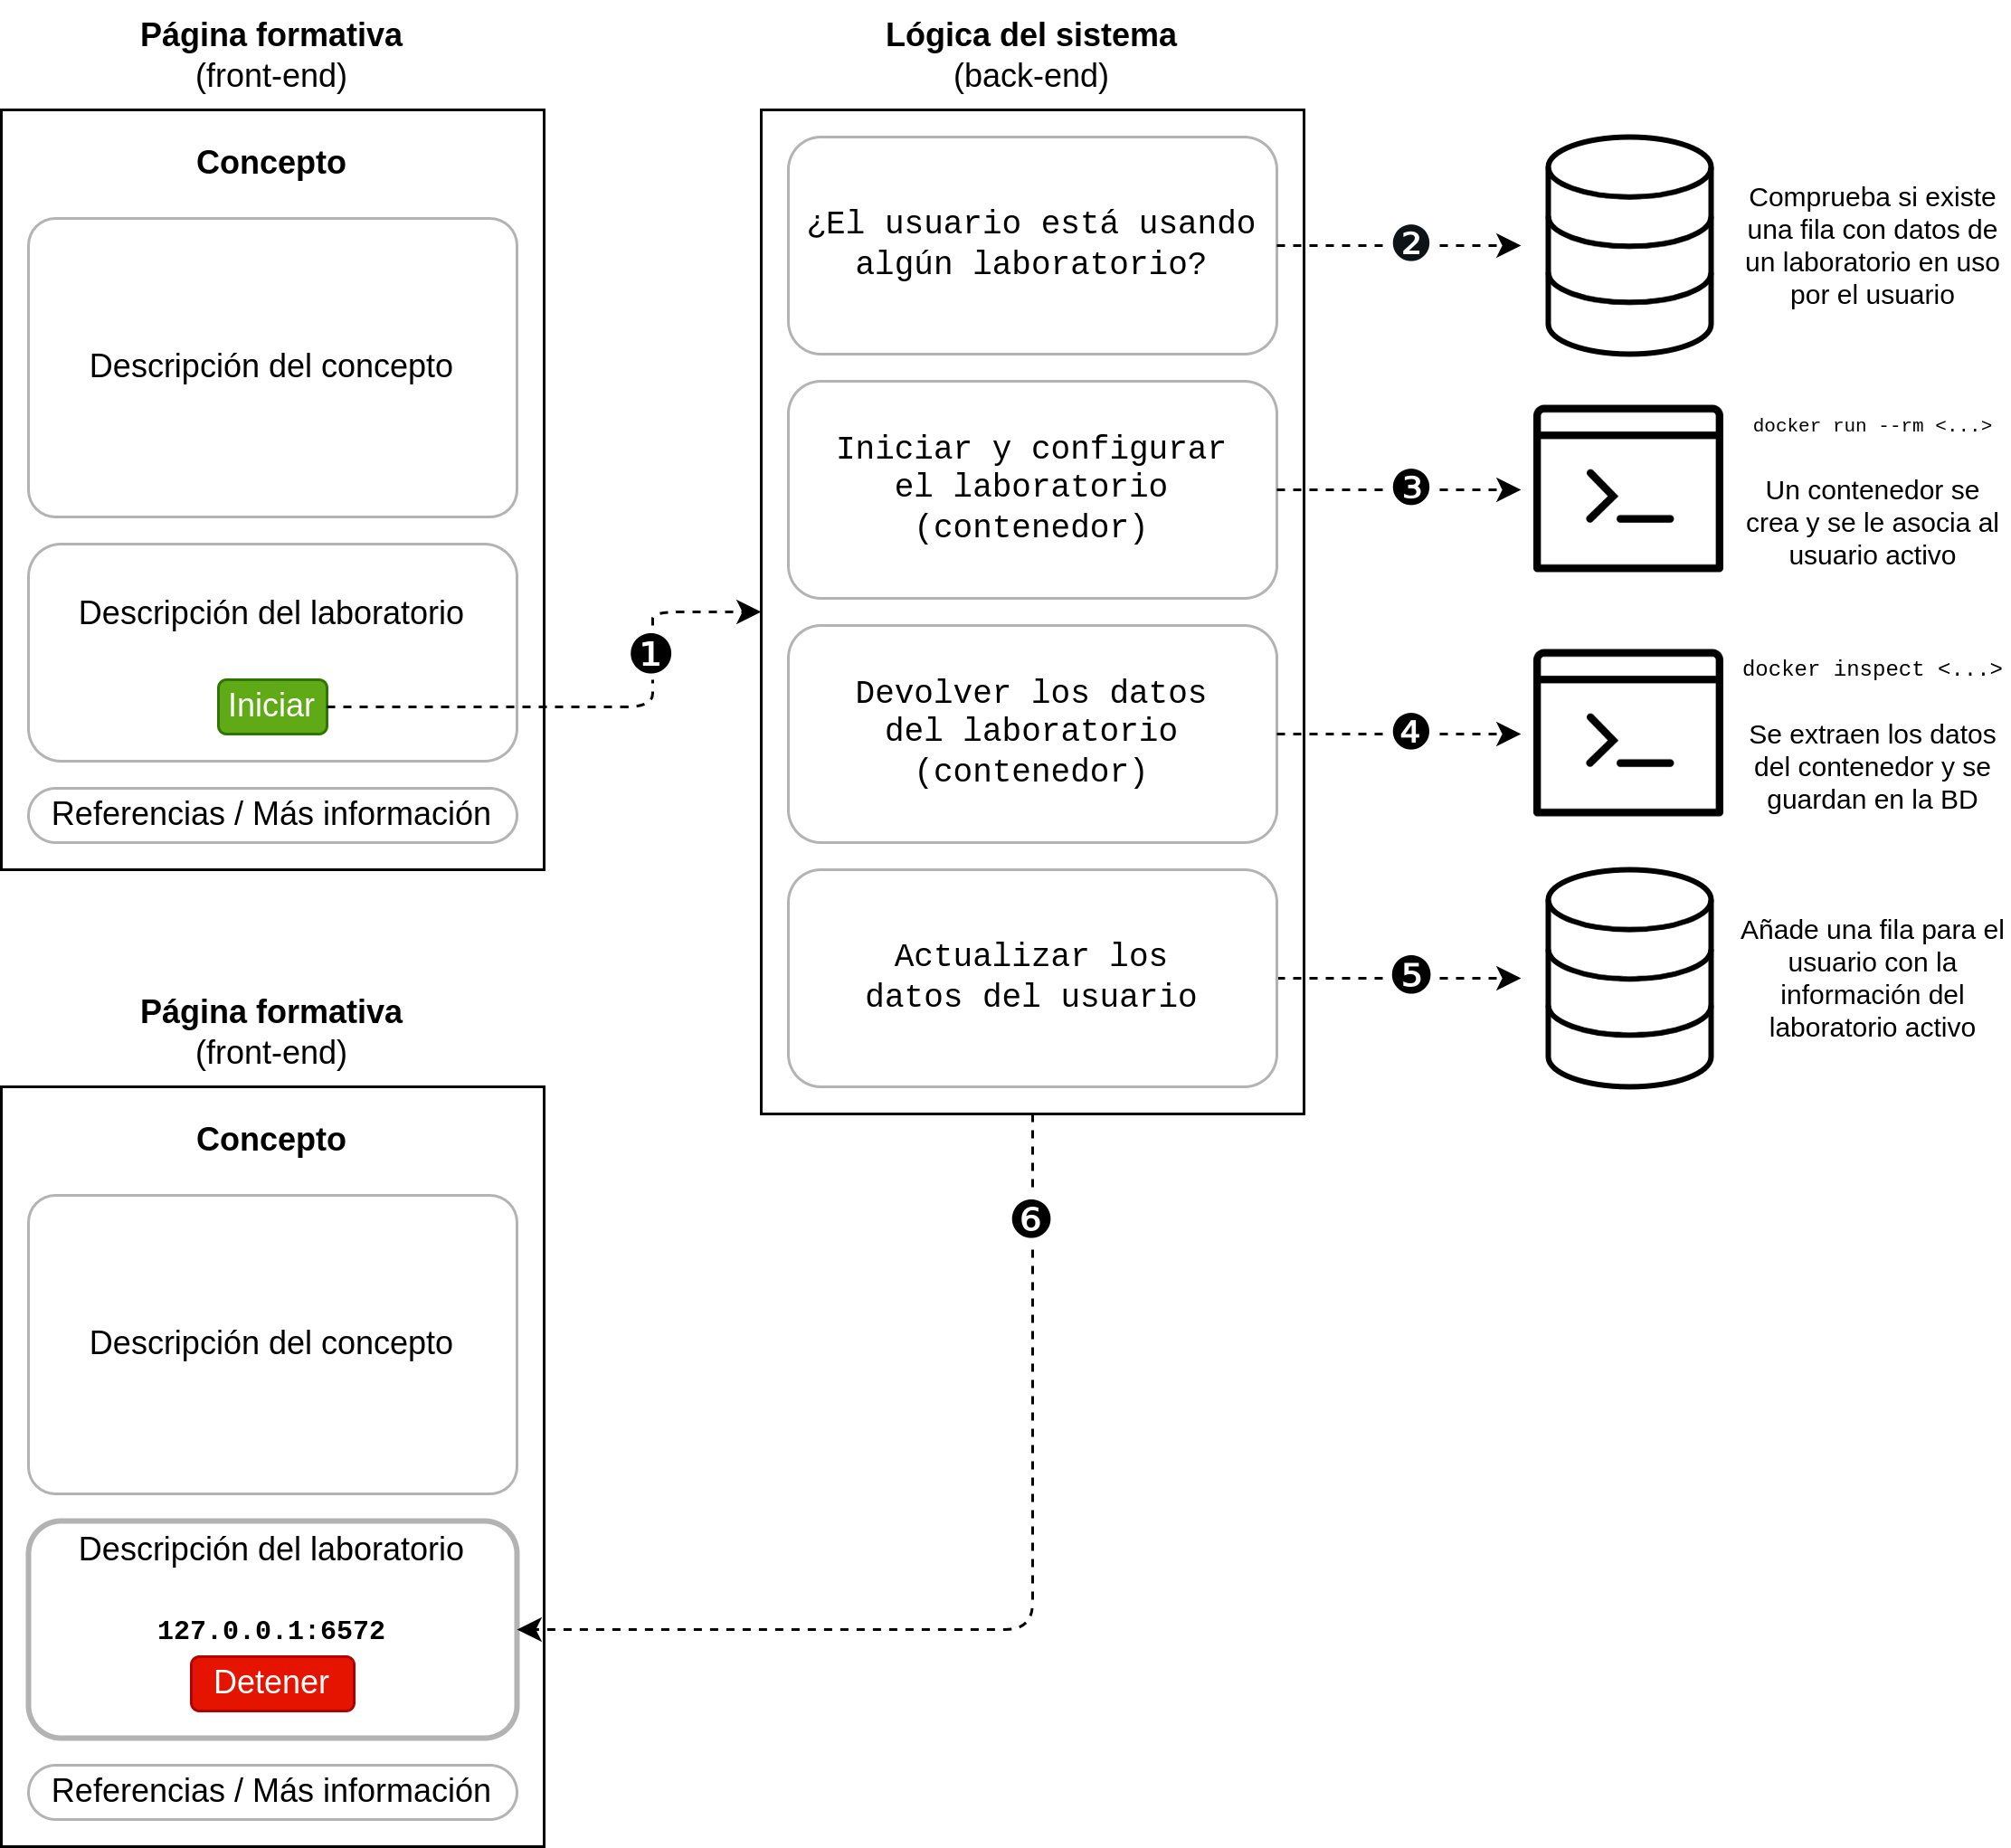
\includegraphics[scale=0.09]{images/diagramas/iniciar.png}
    \end{frame}

    \begin{frame}
        \centering

        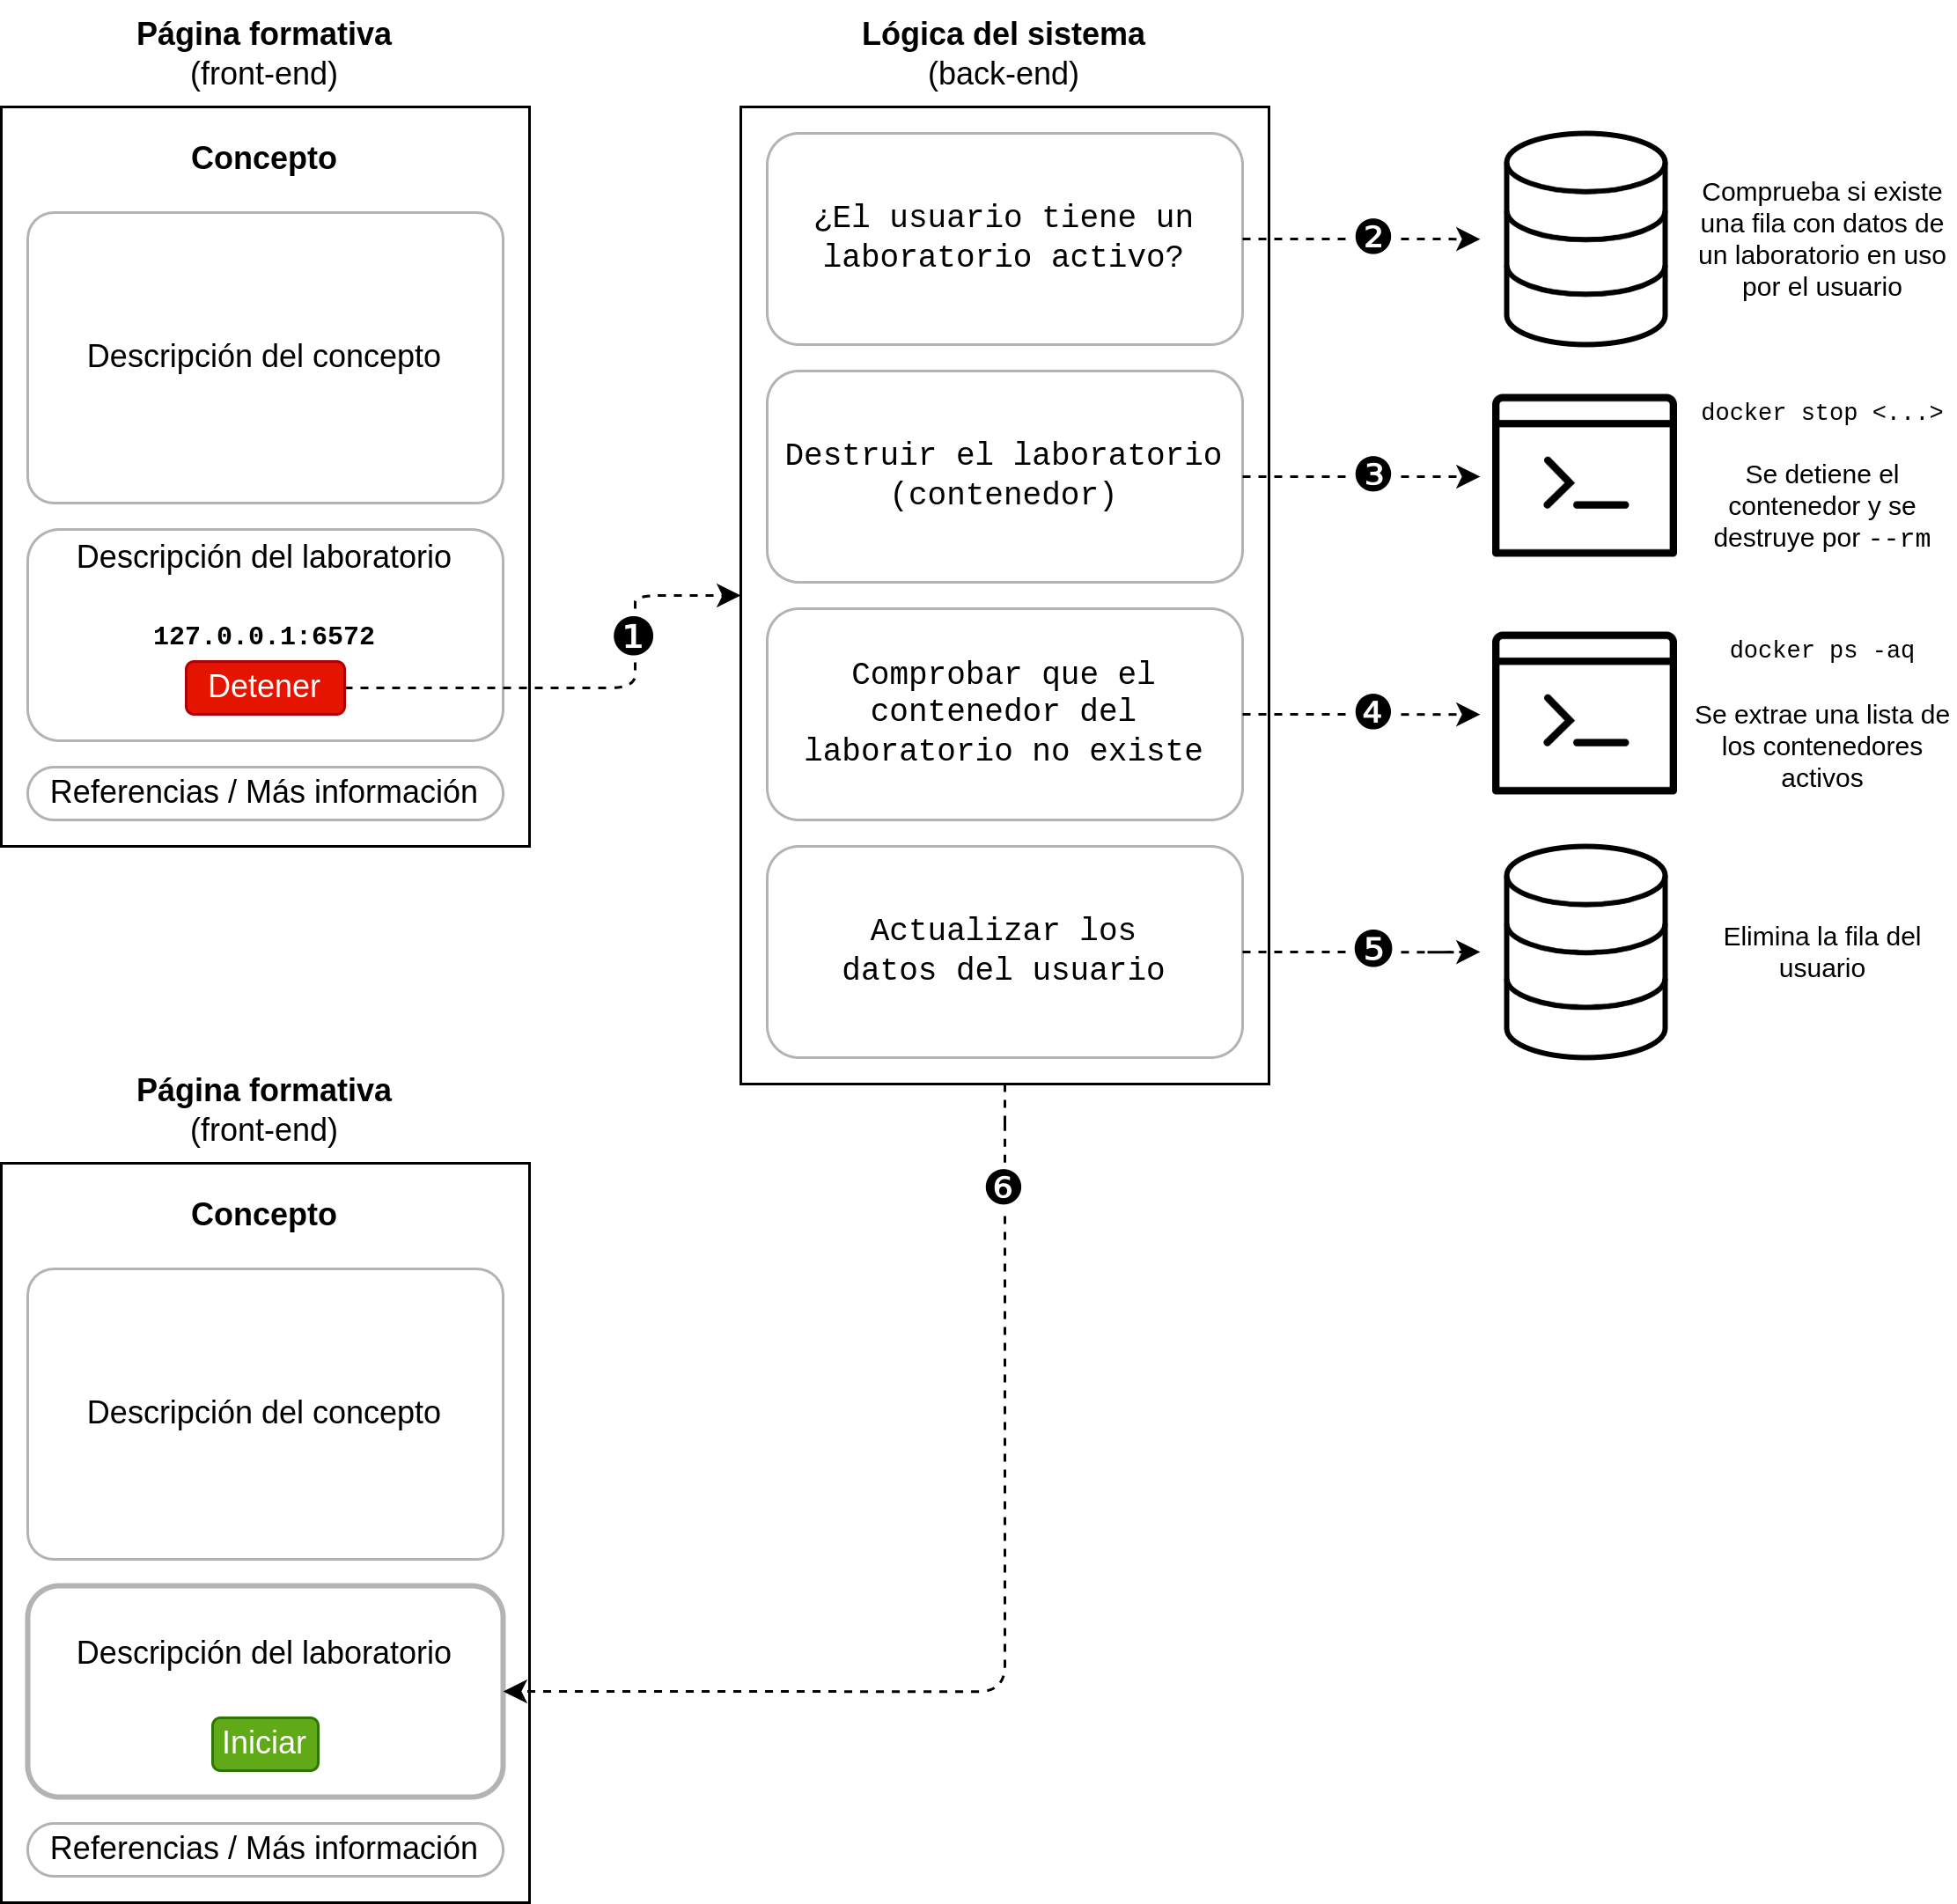
\includegraphics[scale=0.09]{images/diagramas/detener.png}
    \end{frame}

    \begin{frame}
        \centering

        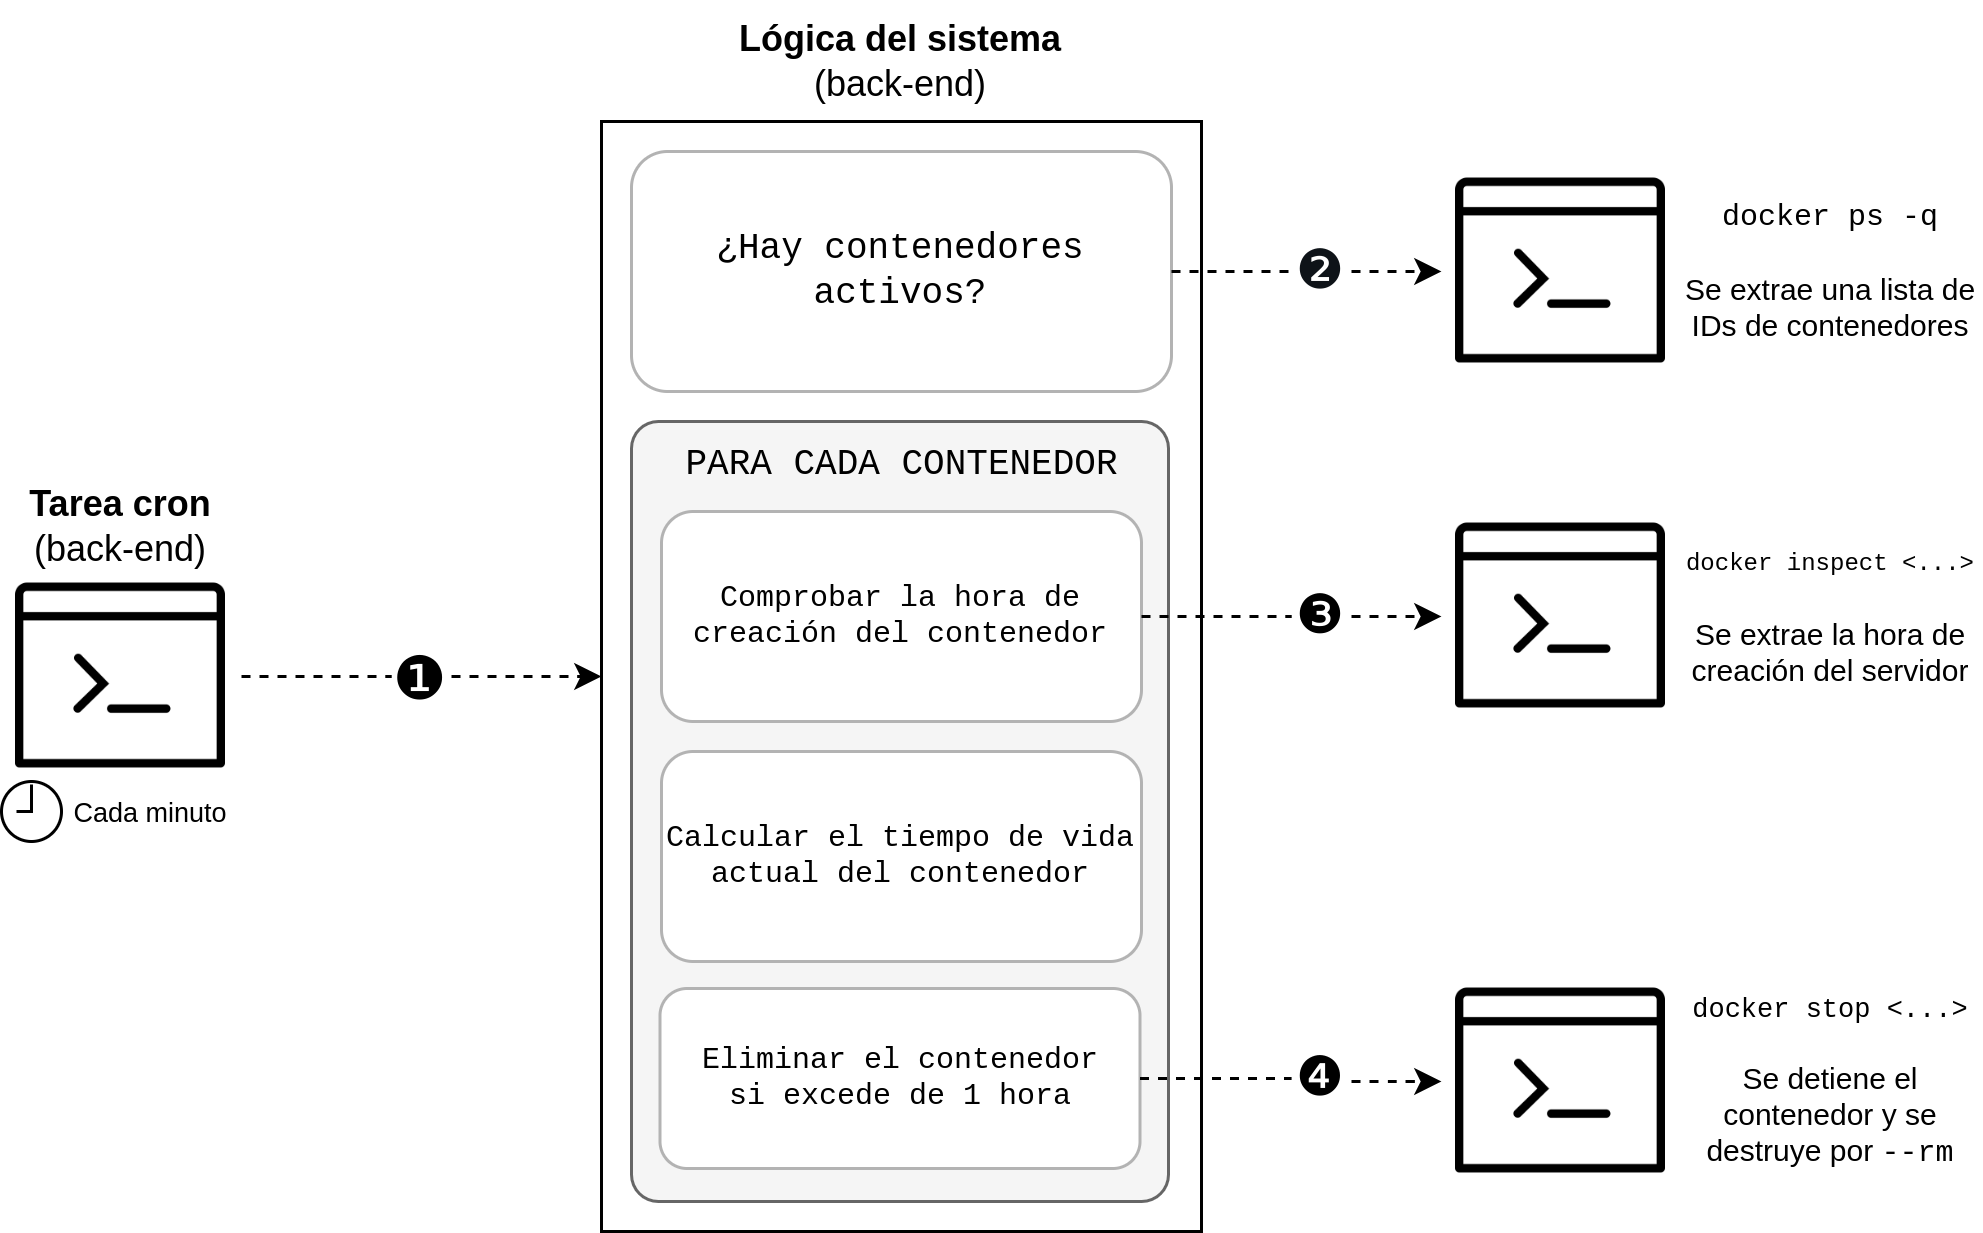
\includegraphics[scale=0.15]{images/diagramas/cron.png}
    \end{frame}

    \begin{frame}{Toma de decisiones}
        \begin{columns}[c]
            \column{.5\textwidth}
                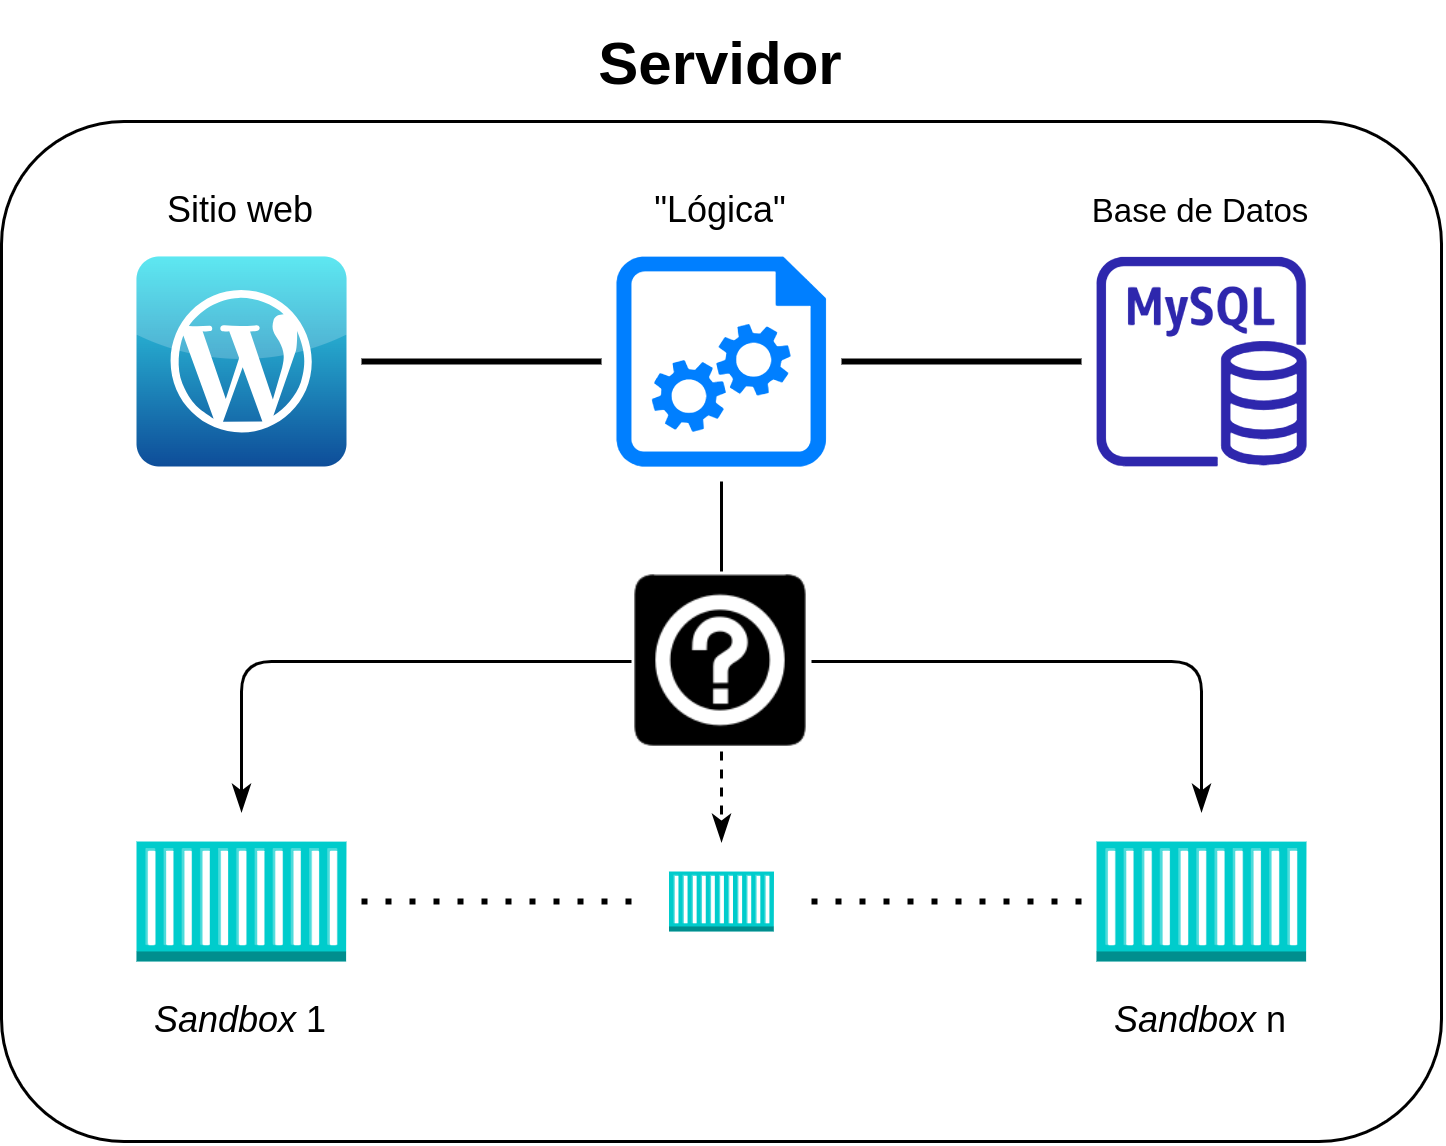
\includegraphics[scale=0.1]{images/diagramas/conexion.png}
            
            \column{.5\textwidth}
                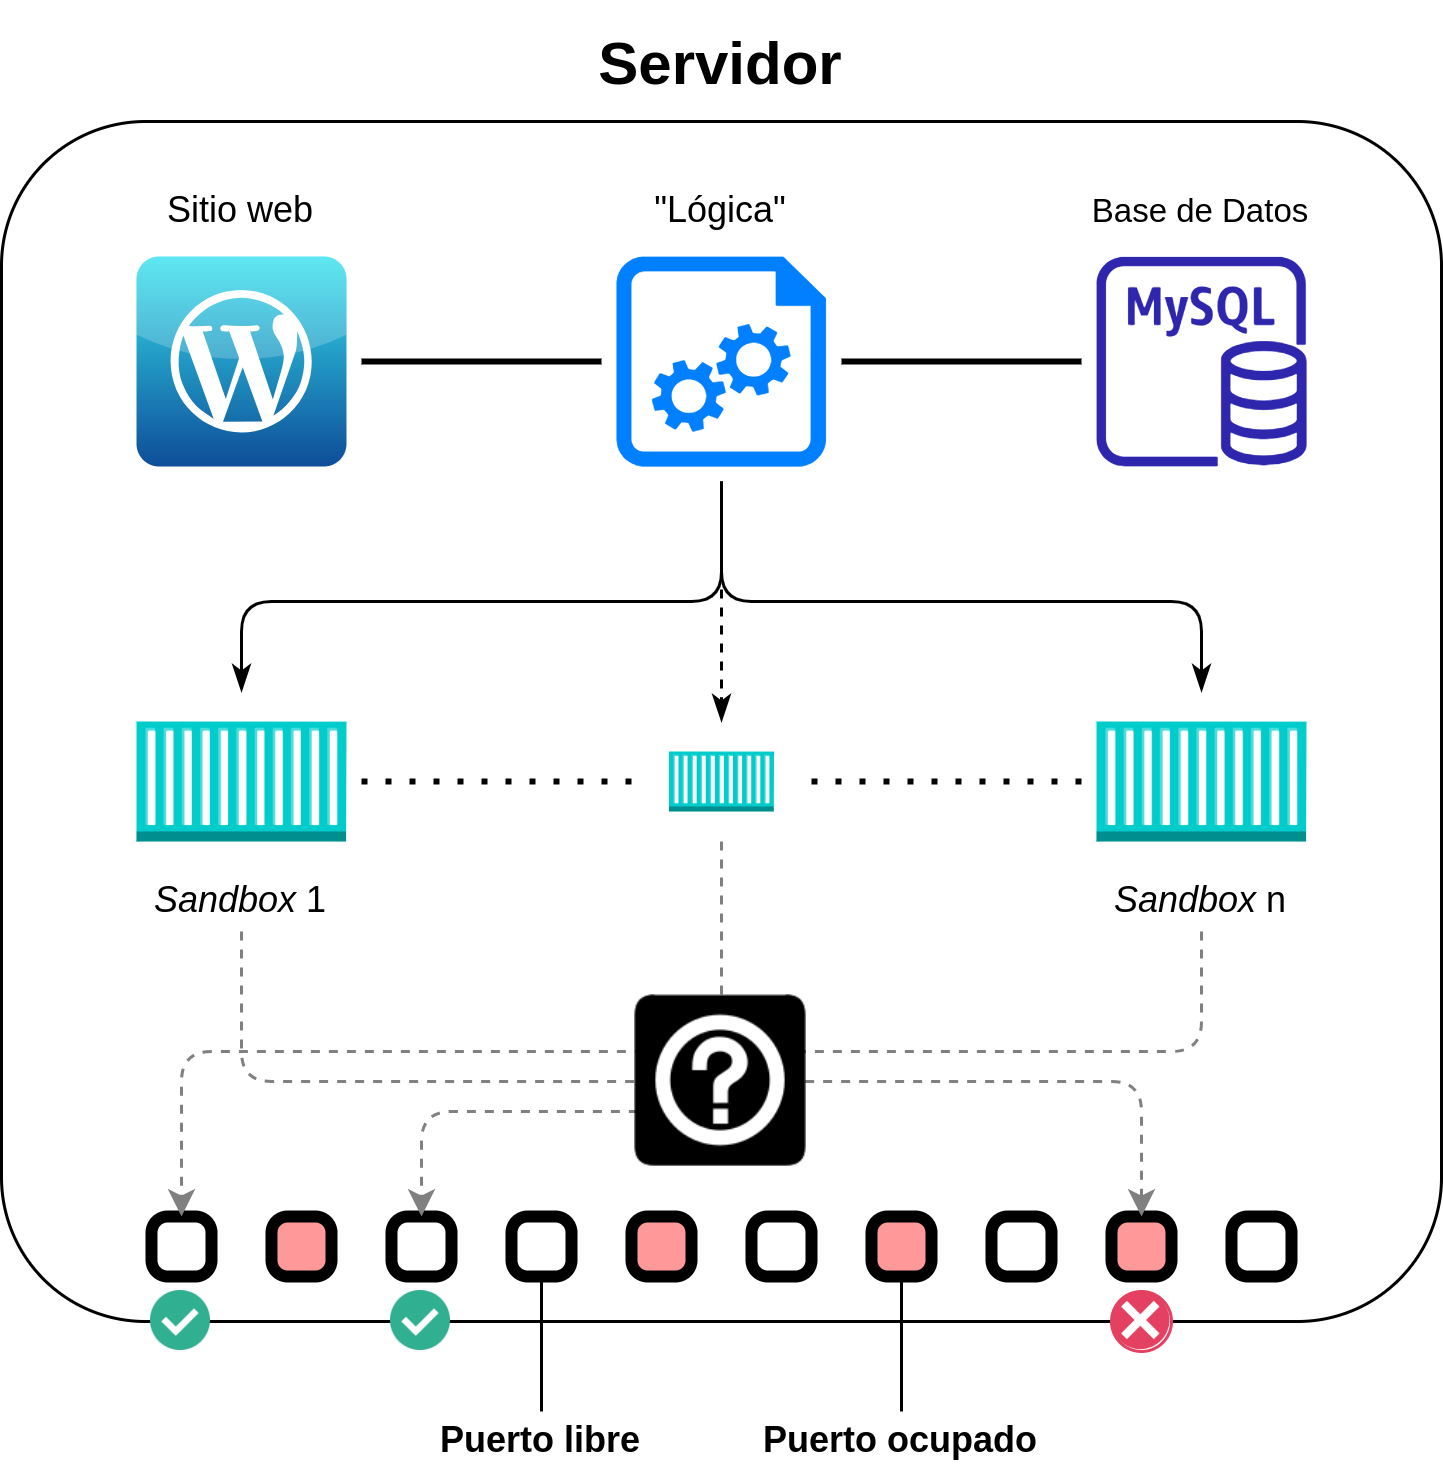
\includegraphics[scale=0.1]{images/diagramas/puertos.png}
        \end{columns}
    \end{frame}


\section{Catálogo de conceptos}

    \begin{frame}
        \Huge{\centerline{Catálogo de conceptos}}
    \end{frame}

    \begin{frame}{Laboratorios de introducción}
        \begin{block}{Linux}
            Jerarquía de ficheros y directorios, y gestión de usuarios y permisos.
        \end{block}
        \begin{block}{Bash}
            Sintaxis básica, variables, condicionantes, bucles y funciones.
        \end{block}

        \begin{block}{Redes}
            Protocolos, tipos y topologías de red, y ataques más comunes.
        \end{block}

        \begin{block}{OSINT}
            Descripción y herramientas útiles de recolección de información.
        \end{block}
    \end{frame}
    
    \begin{frame}{Laboratorios normales}
        \begin{block}{Análisis de tráfico}
            Captura de tráfico, paquetes y herramientas.
        \end{block}

        \begin{block}{Esteganografía}
            Definición y herramientas comunes.
        \end{block}

        \begin{block}{Fuerza bruta}
            Definición y puesta en práctica.
        \end{block}

        \begin{block}{Hash-cracking}
            Descripción y herramientas comunes.
        \end{block}
    \end{frame}
    
    \begin{frame}
        \begin{block}{Criptografía}
            Tipos de cifrado y clasificación, y herramientas criptográficas.
        \end{block}

        \begin{block}{Escalada de privilegios}
            Descripción y casos de uso.
        \end{block}

        \begin{block}{Bypass}
            Descripción a través de la vulnerabilidad CVE-2017-8386.
        \end{block}

        \begin{block}{Ransomware}
            Prueba de concepto de un ransomware.
        \end{block}
    \end{frame}

    
\section{Código auxiliar}

    \begin{frame}
        \Huge{\centerline{Código auxiliar}}
    \end{frame}

    \begin{frame}{Scripts de despliegue}
        \begin{columns}[c]
            \column{.55\textwidth}
                \begin{block}{\texttt{instalar.sh}}
                    \begin{enumerate}
                        \item Obtiene los laboratorios.
                        \item Para cada uno:
                        \item Si ya existe, lo actualiza.
                        \item Si no existe, lo construye.
                    \end{enumerate}
                \end{block}
            
            \column{.45\textwidth}
                
\includegraphics[scale=0.2]{images/capturas/instalar.png}
        \end{columns}
    \end{frame}

    \begin{frame}
        \begin{columns}[c]
            \column{.45\textwidth}
                \begin{block}{\texttt{stop-1h-container.sh}}
                    \scriptsize

                    \begin{enumerate}
                        \item {Obtiene los laboratorios\\activos y su inicio.}
                        \item Para cada uno:
                        \item Muestra un mensaje informativo.
                        \item Si pasó 1 hora, lo destruye.
                    \end{enumerate}
                \end{block}
            
            \column{.55\textwidth}
                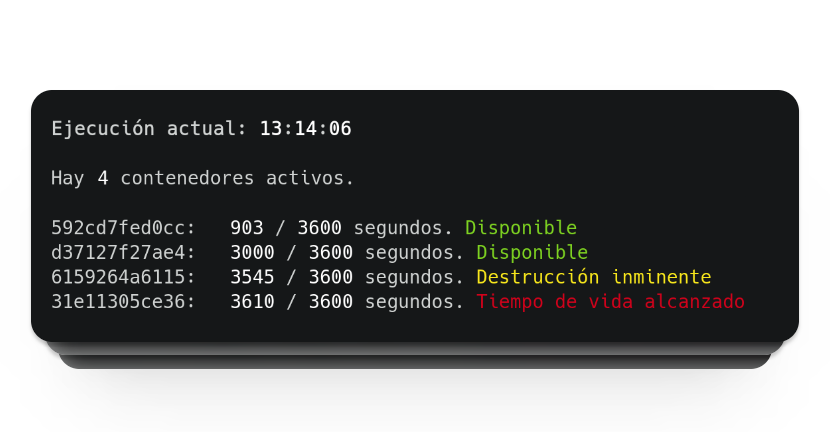
\includegraphics[scale=0.2]{images/capturas/cron.png}
        \end{columns}
    \end{frame}

    \begin{frame}{Proyectos para laboratorios}
        \begin{block}{\texttt{ip-osint}}
            Proyecto escrito en Python que recibe una IP o lista de IPs y devuelve información sobre ellas obtenidas de diversas fuentes.
        \end{block}
        
        \begin{block}{\texttt{stockholm.py}}
            Script escrito en Python que cifra (y descifra) los ficheros de un directorio específico del sistema, simulando un ransomware.
        \end{block}
    \end{frame}


\section{Conclusiones}

    \begin{frame}
        \Huge{\centerline{Conclusiones y futuras}}
        \Huge{\centerline{líneas de trabajo}}
    \end{frame}

    \begin{frame}{Conclusiones}
        \begin{enumerate}
            \item Aumentar mi conocimiento en ciberseguridad
            \\~\\
            \item Aprender sobre Docker y sus posibilidades
            \\~\\
        \end{enumerate}

        \begin{itemize}
            \item Aprender sobre desarrollo web mediante WordPress
        \end{itemize}
    \end{frame}

    \begin{frame}{Futuras líneas de trabajo}
        \begin{itemize}
            \item Trasladar el proyecto a un servicio de alojamiento
            \\~\\
            \item Expandir el contenido de Pentesting
            \\~\\
            \item Optimizar la plataforma (no usar WordPress)
            \\~\\
            \item Generalizar el cotenido (no solo Pentesting)
            \\~\\
            \item Organizar el contenido (categorías, rutas, módulos...)
        \end{itemize}
    \end{frame}

    \begin{frame}
        \Huge{\centerline{Muchas gracias}}
    \end{frame}


\end{document}
